\subsection{Lasso regression}

Our last selection method is the lasso regression. In \Fig~\ref{fig:LassoCoefVsLambda} is shown the coefficients' behavior as $\lambda$ increases. 

The identical procedure utilized for ridge regression is once again implemented. \Fig~\ref{fig:LassoCvPlot} displays the trend of cross-validated MSE as $\lambda$ increases. The optimal value, $\lambda_{opt} = 0.0036$, was identified, which does not enforce any regressor's coefficients to become zero. Similar to ridge regression, no variable selection is conducted in this case as well.

\begin{figure}[H]
	\centering
	\begin{subfigure}{.5\textwidth}
		\centering
		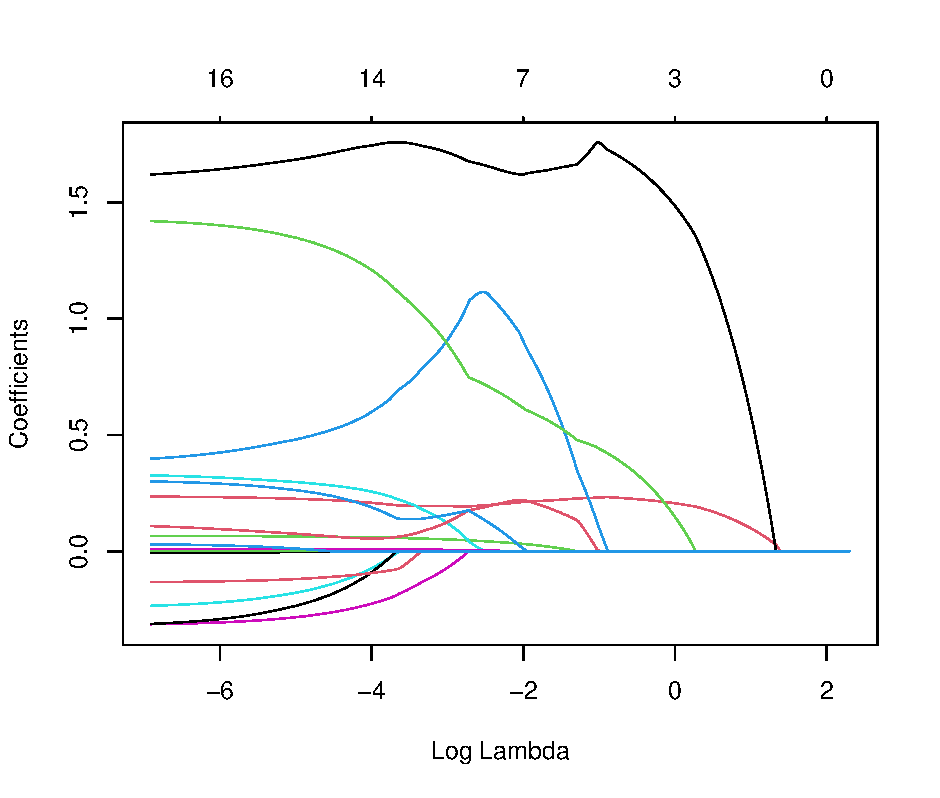
\includegraphics[width=0.7\linewidth]{ImageFiles/Regression/Lasso/LassoCoefVsLambda.pdf}
		\caption{}
		\label{fig:LassoCoefVsLambda}
	\end{subfigure}%
	\begin{subfigure}{.5\textwidth}
		\centering
		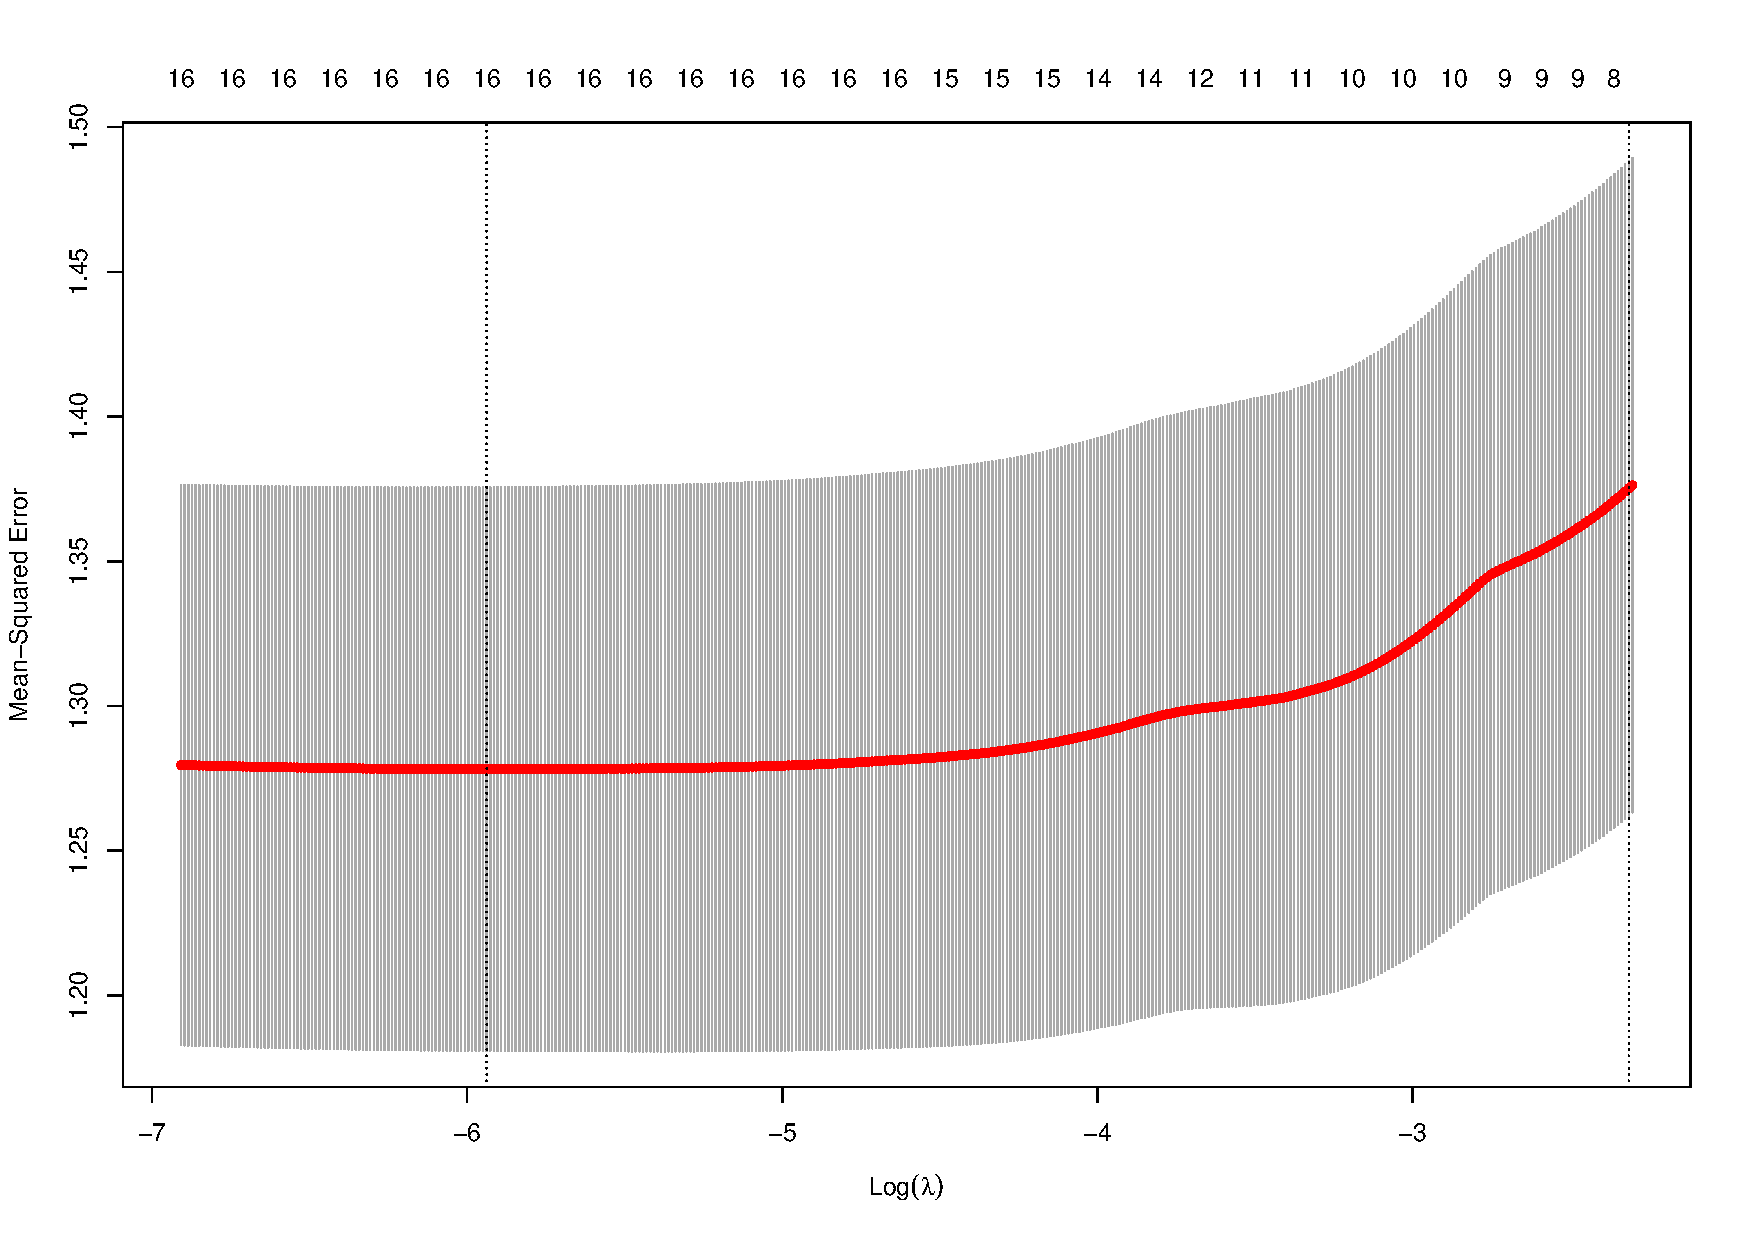
\includegraphics[width=0.7\linewidth]{ImageFiles/Regression/Lasso/LassoCvPlot.pdf}
		\caption{}
		\label{fig:LassoCvPlot}
	\end{subfigure}	
	\caption{Application of lasso regression with different values of $\lambda$. (a) Coefficients as a function of $\lambda$. (b) Cross-validation MSE as a function of $\lambda$.}
	\label{fig:FinalFSSM}
\end{figure}

Upon fitting the model with $\lambda_{opt}$, the resulting coefficients are presented in \Tab~\ref{table:FinalLassoCoef}. The MSE computed for this model is 1.2544.
